Den eigentlichen Beginn dieser Arbeit soll nun eine Ausarbeitung des Problemfelds machen. Es handelt sich um ein sehr umfangreichen Themenkomplex, welcher durch die kurze einleitende Beschreibung nicht komplett zu erfassen ist. Teil dieser Arbeit ist es deshalb an dieser Stelle zunächst zu analysieren, in welchen Kontext die Problemstellung einzuordnen ist und auch genauer zu erarbeiten, welche Dimensionen dort hineinspielen. Es sollen also Details des Problems herausgearbeitet werden und daraus mögliche Potenziale und Ansätze für die nachfolgende Optimierung erkannt werden.

\subsection{Verwandte Arbeiten} 
\todo{Aus Expose kopiert, nochmal überarbeiten?}

Die Problemstellung stellte sich schon bei erster genauerer Betrachtung als durchaus komplex heraus. Das Thema Zeitslotplanung ist im gesamten Bereich Logistik und sogar darüber hinaus von Bedeutung, es gibt somit schon viel Vorarbeit und Literatur in diesem Bereich. Allerdings sind die Anforderungen und Rahmenbedingungen überall sehr unterschiedlich und es lassen sich kaum allgemeine Lösungen finden. Selbst im Bereich der Hafenlogistik gibt es zwischen verschiedenen Häfen, Terminals und Gütern verschiedenste Verfahren und Regelungen.

Es gibt durchaus einige Arbeiten, die sich in einem ähnlichen Rahmen bewegen, also ebenfalls das Thema Zeitslotmanagement in Zusammenhang mit LKW Abfertigung betrachten. In der Regel geht es dabei eher um die effiziente Vergabe der Slots selbst. Beispielsweise darum, wie ankommende LKW möglichst effizient und ohne Zeitverlust auf spezifische und zweckgebundene Laderampen verteilt werden können (siehe \cite{truckDockAllocation}). Weitere Arbeiten beschäftigen sich sogar noch konkreter mit Zeitslotmanagement im Kontext von Hafenterminals, allerdings für Container (siehe \cite{vergleichbareArbeiten2}, \cite{vergleichbareArbeiten1}). Es gibt auch ein Beispiel zur adaptiven Planung von Zeitfenstern, basierend auf Echtzeitdaten der LKW (siehe \cite{vergleichbareArbeiten3}). 

Die meisten dieser Arbeiten beschäftigen sich direkt mit der Planung und Vergabe der Slots selbst. Die Optimierung dieser Arbeit soll hauptsächlich innerhalb dieser Slots stattfinden. Bei der Zeitplanung wird sehr auf die Wünsche der Speditionen eingegangen und es gibt im hier betrachteten Beispiel auch keinen so klar strukturierten Produktionsprozess gibt, wie es möglicherweise in anderer, zuvor genannter Literatur der Fall ist. Der Fokus soll eher darauf liegen, den Lade- und Abladeprozess selbst zu verbessern. Durch verbesserte Verteilung und Sortierung innerhalb des Slots können die in dem Prozess benötigten Ressourcen womöglich besser ausgenutzt werden und so mehr LKW in der gleichen Zeit abgefertigt werden.


\subsection{Ausgangszustand vor dieser Arbeit}

Bei dem hier bearbeiteten Thema handelt es sich um eine sehr spezifische Problematik. In dieser Form gibt es also keine direkten Quellen, auf die aufgebaut werden könnte und aus denen eine Grundlage für die weitere Arbeit gezogen werden kann. Da hier eine Lösung für die spezifischen Softwareprojekte der HEC für die Terminals von Unikai und BLG in Hamburg und Bremerhaven geschaffen werden soll, wurde die folgende Ausarbeitung stattdessen auf Basis von Experteninterviews durchgeführt (siehe Anhang \ref{sec:appendixInterviews}\todo{richtiger Verweis}). Außerdem wurde die bisher eingesetzte Software über einen für diese Arbeit zur Verfügung gestellten Testzugang genauer begutachtet. 

\subsubsection{Aktueller Bearbeitungsprozess}

Prinzipiell teilt sich der ganze Bearbeitungsprozess eines LKW in zwei wesentliche Abschnitte. Zunächst einmal gibt es eine Reihe von Schritten, die ablaufen müssen, bevor ein LKW physisch im Hafen ankommt. Im allerersten Schritt gibt es eine Vorankündigung der Liefergüter. Die sogenannte Avise wird durch die Reeder, also die Eigentümer bzw. Betreiber der Schiffe angemeldet. Durch diese Avise erhält das Terminal schon einmal grundlegende Informationen zu den Gütern, welche zukünftig den Hafen durchlaufen werden. Zu den hier übermittelten Informationen zählt neben einer eindeutigen Buchungsnummer zunächst die Angabe um welchen der drei möglichen Warentypen Container, Stückgut oder Fahrzeug es sich handelt. Für Fahrzeuge und Container werden hier auch Informationen zu den genauen Warenpositionen, also Fahrzeugidentifikationsnummer (FIN) oder Containernummer und ISO-Nummer las Angabe der Containergröße übergeben. Für Stückgüter, welche den Hauptfokus dieser Arbeit darstellen, gibt es keine genauen Angaben zu den Packstücken. Hier kann es mehrere Packstücke unterschiedlicher Art geben, z.B. einen zerlegten Raupenkran. Außerdem werden durch den Reeder noch Ankunfts- (Expected Time of Arrival, ETA) bzw.Abfahrtszeit (Expected Time of Departure, ETD) des Schiffes gelierfert.

Wollen Speditionen oder Fahrer nun einzelne dieser Güter liefern oder abholen, so können diese dann für zuvor avisierte Güter einen Slot buchen. Dazu geben diese zunächst eindeutige Nummern zur Identifikation der Ware ein, wie FIN oder Buchungsnummer. Anhand dessen kann zunächst geprüft werden, ob bereits eine Avise durch den Reeder erfolgt ist. Im positiven Fall können nun noch einmal spezielle Informationen zu den auf dem LKW befindlichen Gütern angegeben werden. Dies können Anzahl, Gewicht oder Maße sein, aber auch Zusatzinformationen, u.a. ob es sich beispielsweise um Gefahrgut oder Zollware handelt. Im Anschluss daran kann ein verfügbarer Zeitslot gewählt werden. Die Verfügbarkeit richtet sich dabei nach mehreren Faktoren. Einmal muss die Ware bis zu einen Tag vor Abfahrt bzw. ab einen Tag nach Ankunft des Schiffes geliefert bzw. abgeholt werden. Außerdem werden bereits hier Abfertiungsbereiche für die spätere Be- und Entladung ermittelt. Jeder Bereich hat hier einen maximalen Vorlauf, wie weit im Voraus gebucht werden kann. In Kombination mit der Anzahl der bereits gebuchten LKW werden aus all diesen Faktoren die verfügbaren Slots angezeigt. Die Anzahl von möglichen LKW pro Slot wird dabei aus Erfahrungswerten bestimmt. Eine Variation über den Tag wird hier auch nur über Erfahrungswerte zu z.B. Pausenzeiten vorgenommen, in denen weniger LKW schaffbar sind. Grundsätzlich wird in den hier betrachteten Terminals mit einstündigen Slots gearbeitet, wobei die Anzahl der LKW die in den Abfertigungsbereichen in dieser Zeit geschafft werden sehr stark schwankt. Die Verfügbarkeit von Laderessourcen unterscheidet sich je nach Bereich sehr und auch die Zeiten für jeden Gütertyp. So lassen sich Container oft sehr schnell abarbeiten, während Stückgüter schon einmal sehr viel Zeit in Anspruch nehmen können und Fahrzeuge liegen zeitlich dazwischen.

Nach erfolgter Anmeldung kann der LKW Fahrer dann zu einem beliebigen Zeitpunkt innerhalb des ausgewählten Slots im Terminal erscheinen und die angekündigte Ware anliefern oder abholen.
\todo{Nach Interview Claas}

\subsubsection{Aktuell genutzte Software}

% - Slotsystem mit festen 1h Slots
% - Eingabemaske für grobe Daten zur Lieferung: Sendungsnr, Größe, Gewicht, Freitextbeschreibung, ...?
% - Wie werden die Daten gespeichert und weiterverarbeitet?
% - Wie wird die Reihenfolge aktuell festgelegt?

Momentan wird eine durch die Firma HEC entwickelte Software eingesetzt und ermöglicht eine Slotbuchung und -steuerung. Sie ist einmal als Desktop Variante verfügbar, was hauptsächlich von Spediteuren genutzt wird. Eine Mobile App kann von LKW Fahrern genutzt werden, um auch unterwegs entsprechende Daten mit einem Smartphone übermitteln zu können. Erfasst werden dabei grobe Daten zu der Sendung und den entsprechenden Gütern. Danach können die Nutzer einen verfügbaren Zeitslot auswählen, in dem sie die benannte Ware anliefern, bzw. abholen möchten. 

Über eine Eingabemaske (siehe Abb. \ref{fig:eingabemaske_aktuelles_system}) können Daten zur Buchung bzw. zu den Gütern, welche er laden oder abholen will eingeben. Dazu gehören u.a. die Buchungsnummer, eine Warenbezeichnung, sowie Anzahl, Größe in Länge/Breite/Höhe und Gewicht. Anschließend gibt es die Möglichkeit, einen Slot auszuwählen, in dem der angemeldete LKW kommen möchte und abgefertigt wird.

\begin{figure}[H]
    \centering
    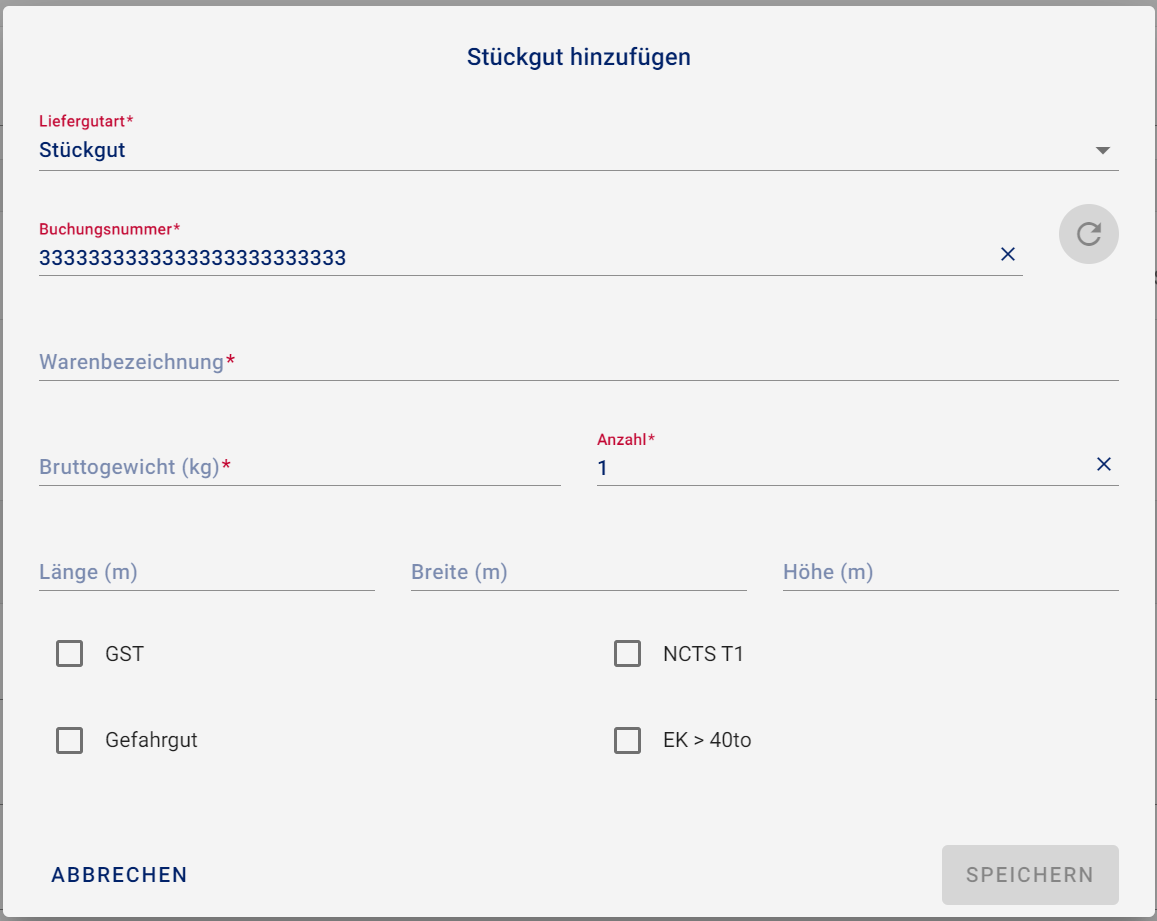
\includegraphics[width=\textwidth]{images/Eingabemaske_aktuelles_System.png}
    \caption[Eingabemaske für LKW Fahrer im aktuell genutzten System]{Eingabemaske für LKW Fahrer im aktuell genutzten System \\ (GST = Großraum- und Schwertransport, NCTS T1 = Zollfreigabe, EK = Einzelkolli/Einzelelement)}
    \label{fig:eingabemaske_aktuelles_system}
\end{figure} 

Alternativ, bzw. ergänzend zur Eingabe über die zuvor beschriebene Anwendung, kann eine Anmeldung automatisiert im EDI-Format erfolgen. Das \glqq{}electronic data interchange\grqq{} Format ist ein standardisiertes Format zum Datenaustausch, welches vor allem in der Schifffahrt noch weit verbreitet ist. Auch hier können erste Daten zum jeweiligen Gut übermittelt werden, ohne eine manuelle Eingabe. Dass das Format standardisiert ist, heißt allerdings auch hier nicht, dass alle übermittelten Daten vollständig und gut sind. Viele Daten, insbesondere die Qualität Beschreibungen hängen auch hier von stark von den bearbeitenden Mitarbeitern ab. \todo{Erklärung/Darstellung EDI und einer Beispiel Message, Quelle?}

Das Terminal hat für das ganze System die Möglichkeit eine Anzahl von LKW einzustellen, welche die jeweiligen Slots buchen und somit belegen können. Diese Anzahl basiert, wie bereits erwähnt, auf Erfahrungswerten. Sie kann stündlich, je nach Verfügbarkeit von Personal, Pausenzeiten o.ä. festgelegt werden. Bei dieser Praxis wird allerdings nicht auf Spezialfälle eingegangen, kommen beispielsweise viele LKW, welche sich schnell abladen lassen, können ungenutzte Leerlaufzeiten entstehen.


\subsubsection{Ablauf der LKW Abfertigung}
\label{sec:analyseAbfertigung}

% - Fahrt zum Ladeplatz -> einer oder mehrere parallel?
% - Varianten von Lademaschinen -> Klassifizierung der möglichen Güter, Zahlen/Grafik zur Häufigkeit
% - Personalverfügbarkeit, Lagerplatz - wovon abhängig?!

Nach seiner Anmeldung muss ein LKW Fahrer innerhalb seines ausgewählten Slots am Terminal erscheinen. Über die von ihm geladenen bzw. abzuholenden Güter wird er dann nach dem \glqq{}First-come-first-serve\grqq{}-Prinzip einem passenden Abfertigungsbereich zugeordnet. Die genaue Ankunftszeit eines LKW innerhalb der gebuchten Stunde ist dabei praktisch eher zufällig. Somit ist es auch hier gut denkbar, dass Leerlaufzeiten entstehen, falls z.B. viele LKW später kommen.

Die Zuordnung eines Abfertigungsbereiches geschieht je nach Ladung des LKW und den dort zur Verfügung stehenden Ladehilfsmitteln. Dadurch, dass es mehrere Ladeplätze gibt, können auch mehrere LKW parallel abgefertigt werden. Je nach Gut werden unterschiedliche Maschinen, Personal und andere Ressourcen benötigt. Es kann auch möglich sein, dass es unterschiedliche Optionen gibt, mit denen ein LKW abgeladen werden kann. So kann möglicherweise ein Kran, aber auch ein Stapler mit passenden Ketten genutzt werden. Hier kann es aber z.B. verschiedene Anfahrts- oder Umrüstzeiten geben. Neben den Ladehilfmitteln und dem Personal ist eine weitere begrenzte Ressource die Stellfläche im Hafen. So kommen die Warenlieferungen idealerweise nicht zu lange vor Abfahrt des Schiffes und gelieferte Waren werden möglichst schnell abgeholt, um Stellfläche für andere Güter freizumachen.

Nach Abschluss des Be- bzw. Entladevorgangs verlässt der LKW das Hafengelände. Der Vorgang ist damit, zumindest auf Sicht der Verladung abgeschlossen.

\todo[inline]{Zuordnung von Hilfmitteln zu Kategorien}

Die im Hafen bearbeiteten Waren lassen sich in folgende wesentliche Kategorien, mit entsprechend genannten Besonderheiten unterteilen:
\begin{itemize}
    \item Container: Standardisiert, evtl. Stellplatz mit Stromanschluss für Temperierung 
    \item Stückgut (z.B. Kisten, Maschinenteile, Kranteile) 
    \item Selbstfahrende Einheiten (z.B. Autos, Zugmaschinen, Kräne): Rollen auf eigener Achse an
    \item Selbstfahrende Einheiten (ebenfalls z.B. Autos, Zugmaschinen, Kräne, landwirtschaftliche Geräte wie Trecker, Mähdrescher): Selbstständiges herunterfahren von anlieferndem Fahrzeug 
    \item Nicht selbstfahrende Einheiten (z.B. Mähdrescher ohne Reifen, Wohnwagen, Eisenbahnwaggons): Abladen z.B. mit Kran 
\end{itemize}

Folgende Ladehilfmittel und Ressourcen werden dabei eingesetzt:
\begin{itemize}
    \item Stapler
    \item Kräne
    \item Reachstacker
    \item Ladegeschirr
    \item Fahrer (von zuvor genannten Maschinen)
    \item Fahrer (für die geladenen Fahrzeuge selbst)
    \item Einweiser
\end{itemize}
\todo{Vervollständigen?!, evtl Bilder zum verdeutlichen?}


\subsubsection{Probleme und Herausforderungen}

Innerhalb des zuvor dargestellten Prozesses gibt es einige Aspekte, welche bisher noch nicht vollumfänglich abgebildet werden konnten, bzw. aktuell noch nicht optimal gelöst sind. Hier ist, insbesondere beim Stückgut, die große Vielfalt an unterschiedlichen Gütern zu nennen. Selten gleicht ein Stück dem anderen und für viele gibt es spezielle Vorgaben und Anforderungen, was deren Handhabung beim Be- oder Entladen angeht. Im bisherigen Vorgehen sind die von den Reedern und Speditionen erfassten Daten oft sehr ungenau oder lückenhaft. Oft werden grobe Warenbeschreibungen wie \glqq{}Maschinenteil\grqq{} übergeben, welche kaum eine Aussagekraft zu den Eigenschaften schlussendlich vorliegenden Gut haben. Eine Bestimmung der Erfassung Anforderungen und somit eine genaue Festlegung der zum Abfertigen des LKWs benötigten Laderessourcen ist dann oft erst bei Ankunft des LKWs im Hafen möglich. Beispielsweise können die exakten Hebepunkte und das dafür benötigte Equipment erst nach menschlicher Begutachtung im Terminal bestimmt werden. Um eine sinnvolle Vorabplanung anstellen zu können, müssten die zum Gut übermittelten Daten sehr viel genauer sein und durch weitere Angaben ergänzt werden. Auch die Vergabe der Slots auf Basis von Erfahrungswerten ist in der Praxis nicht besonders optimal. Durch die große Vielfalt an möglichen Waren ist auch die Menge von gebuchten Gütern sehr unterschiedlich. Es kann sein, dass viele schnelle Aufträge hereinkommen, genauso gut können aber auch viele große und aufwändige Güter in einem Slot kommen.


\subsection{Analyse und Bewertung von Optimierungspotenzialen}
\label{sec:analyseOptimierungspotenziale}

% - Welche Probleme tauchen auf? Z.B. Fahrzeug wechsel und Rüstzeiten dauern lange
% - Macht es Sinn das Slotsystem aufzuweichen und größere/flexible Slots zu machen?
% - Oder einziger Fokus auf Dynamisierung/Verteilung innerhalb eines Slots

\todo[inline]{Später: Diskussion in wie weit diese Optimierungen praxistauglich sind. Wird es in der Praxis möglich sein, Genaue Daten zu bekommen mit denen man planen kann?}

In den Experteninterviews und auch im gesamten vorangegangenen Ausarbeitungsprozess des Ausgangszustands hat sich eine Reihe von Punkten ergeben, die verbesserungswürdig sind und welche bei einer potentiellen Optimierung des gesamten Vorgangs berücksichtigt werden könnten. An vielen Stellen wurden diese in den vorherigen Kapiteln bereits genannt, hier erfolgt nun aber noch einmal eine ausführlichere Auflistung und Analyse dieser Punkte, um mit diesen später ganz konkret weiter arbeiten zu können.

Ein wesentlicher Punkt, welcher weitergehende Optimierungen schwierig macht und welcher vermutlich auch ausschlaggebend dafür war, dass es bisher kaum Anstrengungen zur Verbesserung des Ist-Zustand gab, ist, dass der Umfang und die Qualität der Eingabedaten extrem schlecht ist. Wie bereits erwähnt, werden die Daten bei der Avisierung manuell von Mitarbeitern der Spedition oder vom LKW Fahrer eingegeben. Diese Eingaben sind oft sehr ungenau, oberflächlich oder unvollständig und somit nicht dafür geeignet, eine sinnvolle Planung zu erstellen, bevor die LKW im Terminal ankommen. Genau diese Vorausplanung erscheint aber der einzig sinnvolle Weg zu sein, eine schnellere Abfertigung möglich zu machen. Nur durch gezielte Vorausplanung und einen offline Algorithmus \todo{Quellen?} welcher mit vollständiger Datenbasis arbeiten kann, wird es möglich sein, eine wirklich messbare Verbesserung zu erzielen. Andernfalls wird es bei allen Einflussfaktoren immer ein sehr großer Zufall sein, wenn die LKWs weiterhin so wenig planbar erscheinen. Es wird logischerweise immer nötig sein, die Reihenfolge der Bearbeitung der LKW zu verändern. Wenn dies erst geschehen kann, wenn die LKW im Terminal sind, werden diese zum einen hohe Wartezeiten in Kauf nehmen müssen und zum anderen wird der Spielraum für Verbesserung nicht allzu groß sein, man LKW nicht um viele Stunden verschieben kann und auch bei den nächsten ankommenden eine ähnlich ungewisse Datenlage besteht. Ein wichtiger Schritt zur Verbesserung wird also die klare Definition eindeutig nutzbaren von Eingabedaten sein \todo{Im Fazit erwähnen: Klarere Definition von Eingabedaten umgesetzt}. Fraglich wäre hier allerdings, ob dies praktisch und in Kooperation mit der Vielzahl von Speditionen wirklich so gut umgesetzt werden kann, dass alle oder zumindest nahezu alle Daten gut genug für die weitere Planung sind.

Ein weiterer Ansatz, welcher sicherlich deutliche Zeitverbesserungen erzielen könnte, ist es, die Reihenfolge der LKW derart zu gestalten, dass LKW mit gleichen oder ähnlichen benötigten Ladehilfsmitteln nacheinander bearbeitet werden. Eine eher zufälligen Ankunft der LKW wird in der Regel zu häufigen Wechseln der Hilfmittel und damit auch zu teils großen und wiederkehrenden Wechsel- und Umrüstzeiten führen. Eine geschickte Sortierung der LKW würde dafür sorgen, dass alle LKW mit den gleichen Maschinen auch nacheinander angefertigt werden. Somit müsste bspw. ein Stapler nicht extra nach jedem LKW wegfahren, wenn dieser noch einmal gebraucht wird und könnte schnell alle Aufträge erledigen. Zusätzlicher Vorteil wäre, dass eine Bündelung der Einsatzzeiten der Geräte dafür sorgt, dass diese nicht viele kleine Leerlaufzeiten haben und so evtl. auch an anderer Stelle noch besser ausgenutzt werden können.

Zusätzlich wäre die Auslastung der Ressourcen ein weiteres Optimierungspotenzial. Wenn man bei der Planung der ankommenden LKW nicht nur nach der bloßen Anzahl geht, sondern auch schaut, welche Ressourcen und Hilfsmittel noch frei bzw. wenig ausgelastet sind, könnten diese auch besser ausgelastet werden. Haben sich z.B. schon viele LKW angekündigt, deren Güter per Kran entladen werden müssen, kann der Kran bereits sehr ausgelastet sein, aber die Stapler bspw. noch nicht. Dann könnte der entsprechende Slot z.B. nicht mehr allen Fahrern als frei angezeigt werden, sondern lediglich denen, die mit noch freien Ressourcen bedient werden können. Wenn schon von vorne herein bekannt ist, welcher Auftrag welche Ressourcen benötigt, kann außerdem auch hier eine effizientere Verteilung erfolgen. So könnte auch für weniger Leerlauf und Wartezeiten gesorgt werden.

Ein letzter Aspekt, welcher Einfluss auf die Dauer der Ladevorgänge am Terminal haben könnte, ist die Größe der buchbaren Zeitslots. Größere oder sogar gar keine Slots könnten möglicherweise einen größeren Spielraum bei der Zeitplanung der LKW ermöglichen. Die Idee wäre hier, dass dadurch eine effizientere und passendere Reihenfolge der LKW gefunden werden kann. Auch wenn es aus Terminal-Sicht relativ egal ist, welcher LKW wann kommt, wäre es Sicht der LKW Fahrer und Speditionen die Frage, mit wie viel Spielraum bei der Zeiteinteilung bzw. mit wie viel ungenutzer Wartezeit vor dem Terminal diese zufrieden sind. \todo{Auch im Fazit erwähnen}

%- Größe von Slots ändern, machen größer/kleinere Slots Sinn? Slotsystem ganz aufbrechen?

%- Optimierung von Wechsel/Rüstzeiten etc

%- Verteilung sodass Ressourcen besser ausgelastet werden